\documentclass[tikz, border=5pt]{standalone}

\usepackage{amsmath,amssymb}
\usepackage{xcolor}
\usetikzlibrary{arrows.meta, shadows.blur, shapes.geometric}

\definecolor{utnblue}{RGB}{0, 51, 102}

\begin{document}
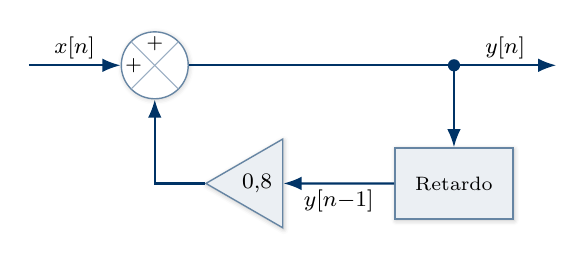
\begin{tikzpicture}[>=Latex, font=\small,
    gain_l/.style={
        regular polygon, regular polygon sides=3, shape border rotate=210,
        draw=utnblue!60, line width=0.5pt, fill=utnblue!8,
        minimum size=1.3cm, inner sep=0pt, font=\footnotesize,
        blur shadow={shadow blur steps=4, shadow blur extra rounding=0pt,
                     shadow xshift=0.4pt, shadow yshift=-0.6pt, shadow opacity=25}
    },
    delay/.style={
        draw=utnblue!60, line width=0.5pt, fill=utnblue!8,
        minimum width=1.5cm, minimum height=0.9cm, font=\scriptsize,
        blur shadow={shadow blur steps=4, shadow blur extra rounding=0pt,
                     shadow xshift=0.4pt, shadow yshift=-0.6pt, shadow opacity=25}
    },
    sum/.style={
        draw=utnblue!60, line width=0.5pt, circle, minimum size=0.85cm,
        inner sep=0pt, fill=white,
        blur shadow={shadow blur steps=4, shadow blur extra rounding=0pt,
                     shadow xshift=0.3pt, shadow yshift=-0.4pt, shadow opacity=20}
    },
    cross_line/.style={utnblue!40, line width=0.4pt},
    signal/.style={->, thick, utnblue},
    wire/.style={-, thick, utnblue},
    tlab/.style={font=\footnotesize, inner sep=2pt, text=black},
]

    \coordinate (in) at (-3.0,0);
    \node[sum] (S) at (-1.4,0) {};
    \draw[cross_line] (-1.4-0.30,-0.30) -- (-1.4+0.30,0.30);
    \draw[cross_line] (-1.4-0.30,0.30) -- (-1.4+0.30,-0.30);
    \node[font=\scriptsize] at (-1.67,0) {$+$};
    \node[font=\scriptsize] at (-1.4,0.27) {$+$};
    \coordinate (tap) at (2.4,0);
    \coordinate (out) at (3.7,0);

    \node[delay]  (D) at (2.4,-1.5) {Retardo};
    \node[gain_l] (g) at (-0.1,-1.5) {$0{,}8$};

    \draw[signal] (in) -- (S.west) node[tlab, above, midway] {$x[n]$};
    \draw[wire]   (S.east) -- (tap);
    \fill[utnblue] (tap) circle (2.2pt);
    \draw[signal] (tap) -- (out) node[tlab, above, midway] {$y[n]$};
    \draw[signal] (tap) -- (D.north);
    \draw[signal] (D.west) -- (g.east) node[tlab, below, midway] {$y[n{-}1]$};
    \draw[signal] (g.west) -| (S.south);

\end{tikzpicture}
\end{document}
